%!TEX root = ../report.tex
\chapter{Methodology}

The Dynamic Motion Primitive is essentially a learning from demonstration (\textit{LfD}) approach for robot programming. To use DMP framework for robotic motion planning and control, following components are needed to be implemented, 

\begin{itemize}
	\item A system for acquiring human demonstrations.
	\item Dynamic motion primitive framework.
	\item Motion controller.
\end{itemize} 

All the methodologies and techniques which are necessary for implementing above mentioned systems, are explained in this chapter. The architecture and implementation details are discussed in the next chapter of this report. 

\section{Dynamic Motion Primitives}

\subsection{Advantages of Dynamic Movement Primitives}
Before diving into the formulation of the dynamic motion primitives, lets summarize the advantages of using them because of which they became the obvious choice for learning control policy.  
\begin{itemize}
	\item It is a model free learning approach.
	\item Any arbitrary trajectory can be learned in end-effector space as well as in joint space.
	\item Here learning is linear regression, so it does not need large dataset.
	One trajectory is sufficient ideally.
	\item Trajectories can be scaled in space as well as in time.
	\item Trajectory evolves as robot actually moves along the trajectory. Hence on-line modifications in the trajectory are possible.
	\item These modifications can be realized by introducing vanishing coupling terms in the differential equations (e.g. potential field around a obstacles \cite{park2008movement}). Perturbations can be handled robustly due to this reason.
	\item Re-planning is not needed unless an event causing major disturbance in the environment occurs.
\end{itemize}

\subsection{Formulation of Dynamic Movement Primitives}

\par Dynamic motion primitives use second order nonlinear differential equations to model motion. These differential equations essentially represent a damped mass spring system where the attractor landscape of differential equations represent desired kinematic states of the robot. Point attractor and limit cyclic behaviors of the second order nonlinear differential equation are used to learn discrete (point to point) and rhythmic robot motion, respectively. Over the time, various versions of DMPs were presented which were slightly different than one another, modified for specific use case or scenario. The following formalization of DMPs is taken from \cite{ijspeert2013dynamical}.

A DMP can be represented by the following set of equations,  
\begin{equation}\label{DMP_1}
\tau\dot{z} = \alpha_{z}(\beta_{z}(g - y) - z) + f(x)
\end{equation}
\begin{equation}\label{DMP_2}
\tau \dot{y} = z
\end{equation}
and the non-linear function $f(x)$
\begin{equation}\label{forcing_term}
f(x) = \frac{\sum_{i=1}^{N}\psi_{i}(x)w_{i}}{\sum_{i=1}^{N}\psi_{i}(x)}x(g - y_{0})
\end{equation}
where,
\begin{equation}\label{psi}
\psi_{i} = \exp(-{\frac{1}{2\sigma_{i}^{2}}(x - c_{i})^{2}})
\end{equation}
and,
\begin{equation}\label{canonical}
\tau \dot{x} = -\alpha_{x}x
\end{equation}

Equation \ref{DMP_1} and \ref{DMP_2} are a first order representation of an autonomous non-linear second-order differential equation where $f(x)$ is a non-linear term. 
Upon solving these equations, we get the state $[\ddot{y}, \dot{y}, y]$ at each time instance. Normally, the Euler's integration method is used to solve this system of equations.  

If the forcing term in eq. \ref{DMP_1} is made 0 i.e. $f = 0$, these equations represent a globally stable second-order linear system with $(z, y) = (0, g)$ as a unique point attractor. "With appropriate value for $\alpha$ and $\beta$ (with $\beta_{z} = \alpha{z}/4$), the system can be made critically damped resulting in $y$ monotonically and asymptotically converging towards $g$"\cite{ijspeert2013dynamical}. Such a system implements a stable but trivial pattern generator with $g$ as single point attractor \cite{ijspeert2013dynamical}.

The idea is to use the eqs. \ref{DMP_1} and \ref{DMP_2} for encoding the control policy to generate kinematic commands for the robot (joint level motion commands or Cartesian motion commands). The kinematic state $[\ddot{y}, \dot{y}, y]$ obtained by solving these equations at each time step, is used as the kinematic commands (position, velocity and acceleration) for the robot manipulator (angular commands for individual joints or Cartesian commands for end-effector), which will become clear later.

With the term $f=0$, evolution of system in eqs. \ref{DMP_1} and \ref{DMP_2} always be of same nature, i.e. $y$ will eventually become $g$ monotonically and asymptotically, given that system is critically damped. By introducing the term $f$, the path followed by the system in attractor landscape of differential equation from initial state to the goal state can be modified arbitrarily. This in-turn modifies the trajectory followed by a mobile robot or a robotic manipulator in the task or joint-space. This non-linear forcing function enables the DMP framework to learn almost any arbitrary motion in end-effector space or joint space. It is essentially a normalized weighted sum of equally spaced Gaussian functions denoted by $\psi$ (eq. \ref{psi}) activated at each time step by the phase variable $x$. The forcing term $f(x)$ is learned from the demonstrated trajectories (discussed in detail in section \ref{learn_DMP}). It should be noted that the forcing term $f$ is modified by the separation between the goal and initial position ($g - y_{0}$), which ensures that the shape of trajectory is also modified by goal separation. Eq. \ref{DMP_1} and \ref{DMP_2} are together called the \textit{transformation system}, as they transform the current state of the system to the next state.   

Equation \ref{canonical} is called the \textit{canonical system}. $x$ acts as a phase variable modifying forcing term $f(x)$ and hence modifying the shape of the trajectory. This removes the explicit time dependency of the $f$, which eliminates the need of maintaining complex timing mechanisms to synchronize multiple DMPs. $x$ initialized at 1 decays to 0 at the end of the motion, which makes $f(x) = 0$ at the end of the motion, ensuring convergence of $y$ to goal state $g$. "It is used to localize the basis functions (i.e., as a phase signal) but also provides an amplitude signal (or a gating term) that ensures that the nonlinearity introduced by the forcing term remains transient due to asymptotical convergence of $x$ to zero at the end of the discrete movement" \cite{ijspeert2013dynamical}.

The term $\tau$ is time scaling factor which can be used to modify the speed of execution of the system by modifying the acceleration and velocity terms. The term $c_i$ in eq. \ref{psi} is the center of $i^{th}$ Gaussian function.    

Similar to the above discussed point attractor behavior, DMPs can also learn rhythmic motions exploiting the limit cyclic behavior of non-linear second order differential equation. To achieve rhythmic motion, we need to a learn forcing term $f(x)$ which is periodic itself and makes the system of equations \ref{DMP_1} and \ref{DMP_2} exhibit limit cyclic behavior. This can be achieved by choosing the canonical system to be,

\begin{equation}
	\tau \dot{\phi} = 1
\end{equation}  

where $\phi \in [0, 2\pi]$ is the phase angle of the oscillator in polar coordinates and the amplitude of the oscillation is assumed to be $r$. Similar to the discrete system, this rhythmic canonical system serves to provide both an amplitude signal $r$ and a phase signal $\phi$ to the forcing term $f$ in equation \ref{DMP_1}:

\begin{equation}
	f(r, \phi) = \frac{\sum_{i=1}^{N}\psi_{i}(x)w_{i}}{\sum_{i=1}^{N}\psi_{i}(x)}r
\end{equation}

\par At this point it becomes clear that the point attractor and limit cyclic behaviors exhibited by non-linear second order differential equation can be used to model discrete (point to point) and rhythmic motions of robotic arm or mobile platform.   
\vspace{0.5cm}

In this project, point attractor DMPs for discrete motion (point-to-point motion) were implemented. For the ease of implementation, above system was slightly modified as follows, 
\begin{equation}\label{actual_DMP}
	\ddot{y} = \tau^{2}(\alpha_{y}(\beta_{y}(g-y)-\dot{y}) + f)
\end{equation}
\begin{equation}
	\dot{x} = \tau(-\alpha_{x}x)
\end{equation}

This modification does'nt change the properties of the original DMP formulation. Unlike the original formulation, the term $\tau^2$ is now multiplied on right side of equation and the first derivative term (velocity) $\dot{y}$ is not multiplied by $\tau$. Still the $\tau$ will affect the speed of evolution of the differential equation system as it scales the acceleration term. 

Figure \ref{fig:DMP_framework} taken from \cite{ijspeert2013dynamical} shows the composition of the DMP framework. The \textit{Coupling Terms} in the figure consists of feedback from the sensors, obstacle coupling terms, error in the execution speed of the DMPs, etc. The canonical system generates the phase variable $x$ at each time step which is used for generating a non-linear forcing term. This forcing term then modifies the behavior of the kinematic motion commands generated by the transformation system. The kinematic motion commands are then executed by robot controller (e.g. velocity controllers, torque controllers, etc.)

\begin{figure}[H]
	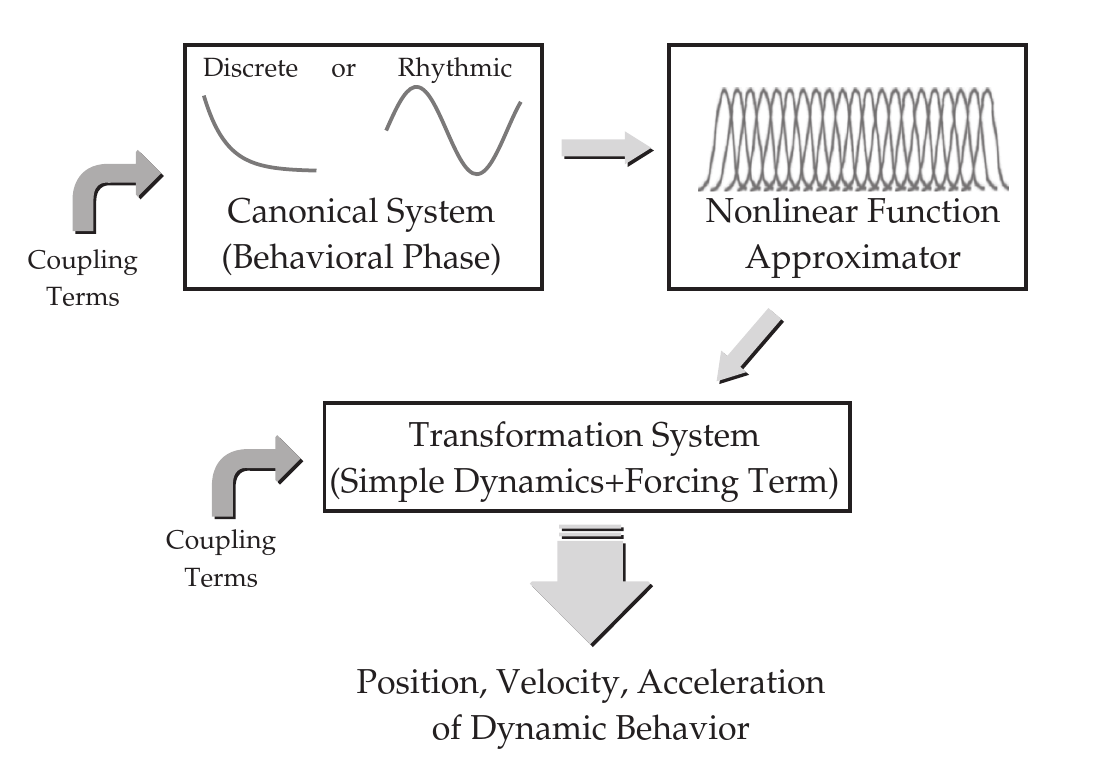
\includegraphics[width=\textwidth]{images/dmp.png}
	\caption{Dynamic Movement Primitive framework \cite{ijspeert2013dynamical}}
	\label{fig:DMP_framework}
\end{figure}
 
\subsubsection{Discussion}

To have an intuitive understanding of the DMP framework, imagine a critically damped mass-spring system, in which a point mass is attached to a spring which is fixed at one end. The length of the spring lie along the Y-axis, making the system strictly one dimensional. Initially, the system is at equilibrium point i.e. spring is not stretched and point mass is at position $g$, the equilibrium point. If the mass is stretched to position $y$ and released, it travels along the Y-axis towards the equilibrium point of the system of i.e. till the spring attains its natural length. Since the system is critically damped, we don't observe any oscillations around the equilibrium point. As mentioned earlier, this system can be mathematically expressed by \ref{DMP_1} and \ref{DMP_2} when $f$ is 0. These equations state the position, velocity and acceleration of point mass at each point in time. Same set of equations which governs the motion of mass-spring system along the Y-axis can be used for encoding manipulator end-effector motion in X-axis, Y-axis and Z-axis, to create a 3-dimensional trajectory. Same set of equations can also encode the motion of single manipulator joint. Use of multiple equations as such, will allow us to encode motion of manipulator in 6 degrees of freedom in task space or the motion of every joint in the joint space. Solving all these equations step by time step, desired kinematic commands can be obtained and passed to robot controllers to be executed. It is also possible to solve these equations till they converge to equilibrium point $g$, which will give us entire trajectory that the end-effector should follow to attain the goal $g$ (goal $g$ will be a goal vector in this case).  

 

\begin{figure}[H]
	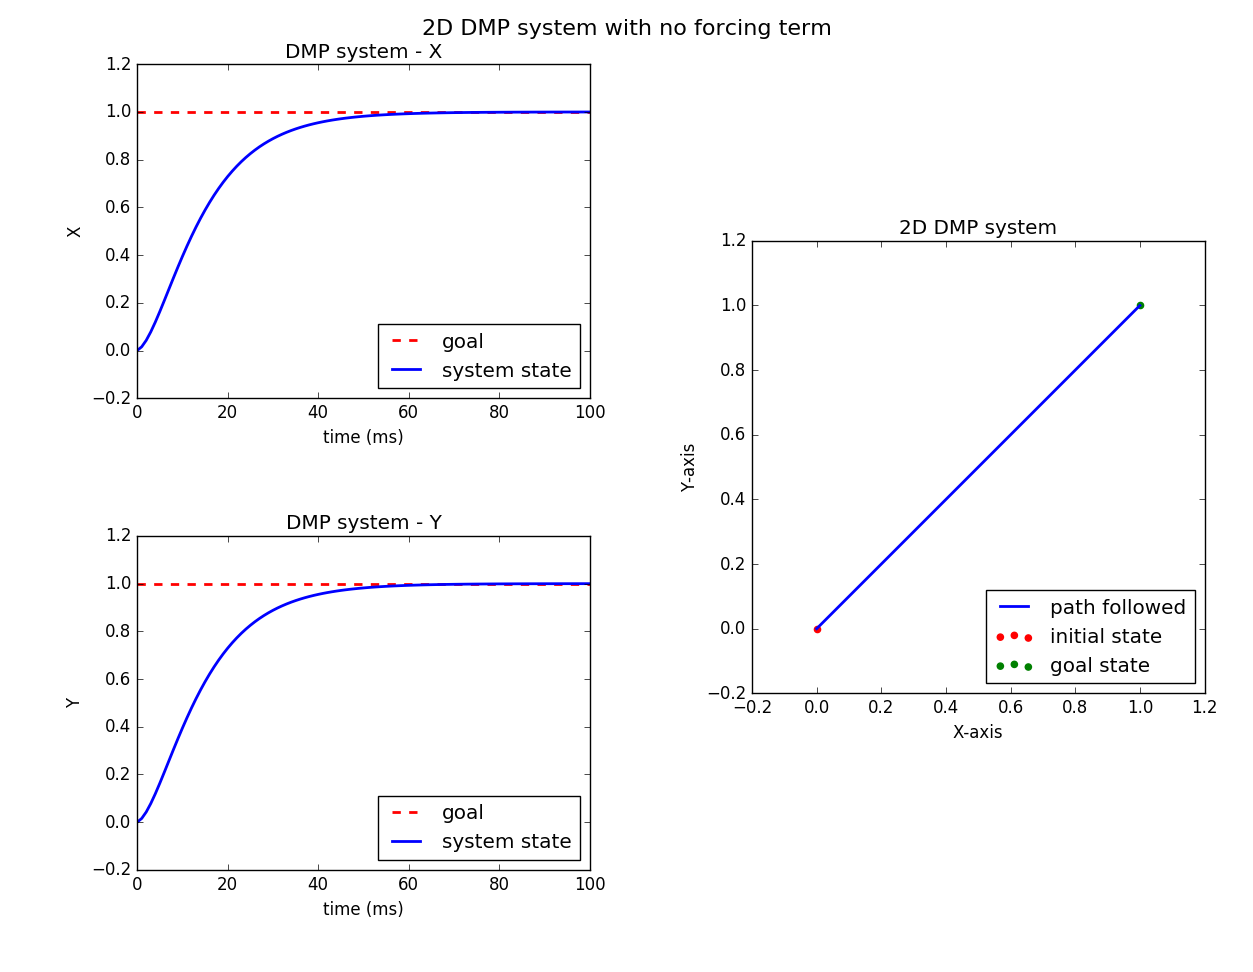
\includegraphics[width=\textwidth]{images/dmp_no_f.png}
	\caption{2D DMP with no forcing term}
	\label{fig:DMP_2DOF}
\end{figure}

Figure \ref{fig:DMP_2DOF} shows the path generated in Cartesian space, by 2 degrees-of-freedom DMP with no forcing term. Figure illustrates the superposition of 2 DMPs in different degrees of freedom. DMP systems in $X$ and $Y$ axes follow the kinematic trajectories same as of damped mass-spring system and superposition of these two motions generate a straight line motion in 2D space. 

But rarely in real world, robots need to follow such straight line path. Numerous robotic tasks demand complex trajectories, and hence we use forcing term $f$ to modify the behavior of trajectory (by adding $f$ to the acceleration at each time step).

Now the question is, do we know the appropriate values of $f$ to add in the acceleration term? No, we don't. But it seems that if we know the values of $w$'s in eq. \ref{forcing_term}, we can estimate the the value of $f$. Again, do we know the appropriate value of $w$'s? And again, we don't. So lets learn them. 

\subsection{Learning the Motion Primitive from Demonstrated Trajectories}\label{learn_DMP}
\par Learning motion primitive implies learning the weights $w_{i}$ in the eq. \ref{forcing_term}. Above system presented in \cite{ijspeert2013dynamical} is linear in the weights $w_{i}$. So variety of learning algorithms can be used. \cite{ijspeert2013dynamical} uses locally weighted regression to learn the weights. 

Desired behavior that should be exhibited by the system is presented as a tuple ($y_{demo}(t)$, $\dot{y}_{demo}(t)$, $\ddot{y}_{demo}(t)$) representing position, velocity and acceleration respectively where $t = [1,2,3,4,....,p]$. Parameter $g$ is goal hence, $g = y_{demo}(t = p)$ and $y_{0} = y_{demo}(t = 0)$. Parameter $\tau$ is temporal scaling factor which needs to be adjusted for achieving desired time scaling in the motion. In order to use LWR for estimating $w_{i}$, eq. (\ref{actual_DMP}) can be rearranged to generate function approximation problem as,
\begin{equation}
f = \ddot{y} - \alpha_{z}(\beta_{z}(g - y) - \dot{y})
\end{equation}

While learning the motion primitives, time scaling factor $\tau$ is set to 1 to ensure learning the motion primitive with same speed as demonstrated. 

By substituting the information from the demonstrated trajectory in the left-hand side of this equation, we obtain,
\begin{equation}
f_{target} = \ddot{y}_{demo} - \alpha_{z}(\beta_{z}(g - y_{demo}) - \tau\dot{y}_{demo})
\end{equation}


As we have the values $f_{target}$, we can perform a supervised learning to find a best fit for the function represented by $f_{target}$. 

Locally weighted regression finds for each kernel function $\psi_{i}$ in $f$, the
corresponding $w_{i}$, which minimizes the locally weighted quadratic error criterion,

\begin{equation}
J_{i} = \sum_{t=1}^{p}\psi_{i}(t)(f_{target}(t)-w_{i}\xi(t))^{2}
\end{equation}

where $\xi_{i} = x(t)(g-y_{0})$ for the discrete system and $\xi_{i} = r$ for rhythmic system. Solution to above linear regression problem is,

\begin{equation}
w = \frac{s^{T}\Gamma_{i}f_{target}}{s^{T}\Gamma_{i}s}
\end{equation}

where,\\
\\
\vspace{1cm}
$
s = 
\begin{pmatrix}
\xi(1) \\
\xi(2) \\
\vdots  \\
\xi(p) 
\end{pmatrix}
$
$
\Gamma = 
\begin{pmatrix}
\psi_{i}(1) &   &  & 0 \\
&\psi_{i}(2)&  &  \\
&  & \ddots &   \\
0 &  &  & \psi_{i}(p)
\end{pmatrix}
$
$
f_{target} = 
\begin{pmatrix}
f_{target}(1) \\
f_{target}(2) \\
\vdots  \\
f_{target}(p) 
\end{pmatrix}
$
\\
and $w$ is the weight vector.  

Learned weights are stored in the library to be used later.


\subsubsection{Discussion}
Now that we know, how to learn weights to generate a forcing function that can enable DMP to learn any arbitrary trajectory, we can discuss the significance of the forcing term $f$. To analyses the roll played by forcing term, lets learn a step function like trajectory in 2D space, shown in the fig. \ref{fig:step_f}.   

Because of the step function like nature of the trajectory, it is interesting to observe the forcing term $f$ associated with the DMP in y-axis, which is shown in fig. \ref{fig:step_f_y}.
\begin{figure}[H]
	\centering
	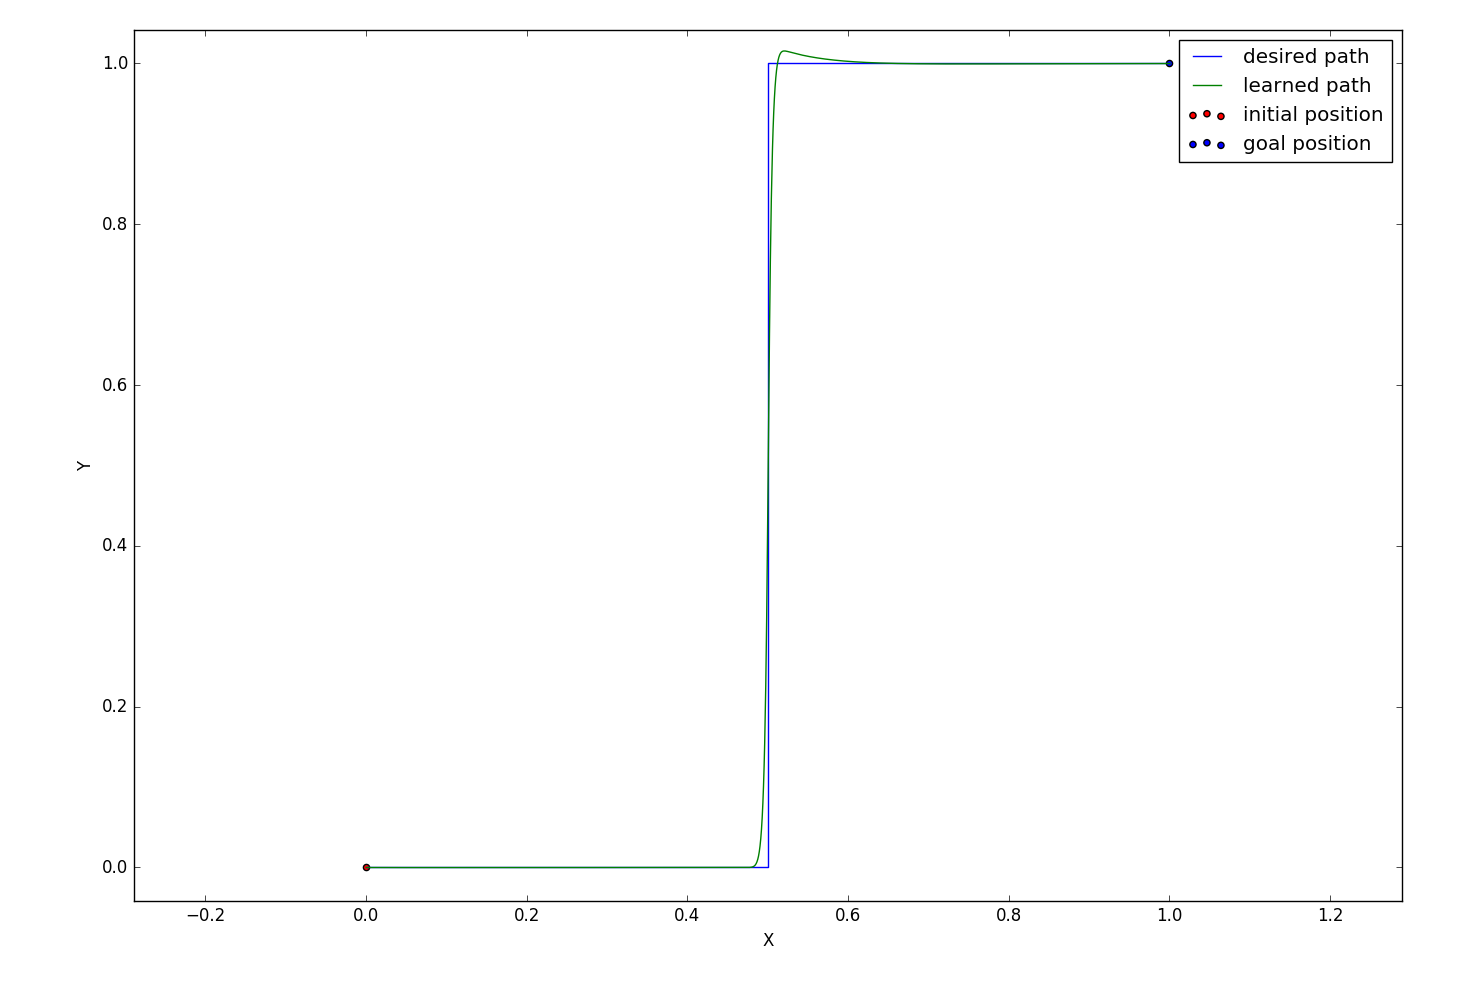
\includegraphics[scale=0.35]{images/step_f.png}
	\caption{Step function trajectory path}
	\label{fig:step_f}
\end{figure}



\begin{figure}[H]
	\centering
	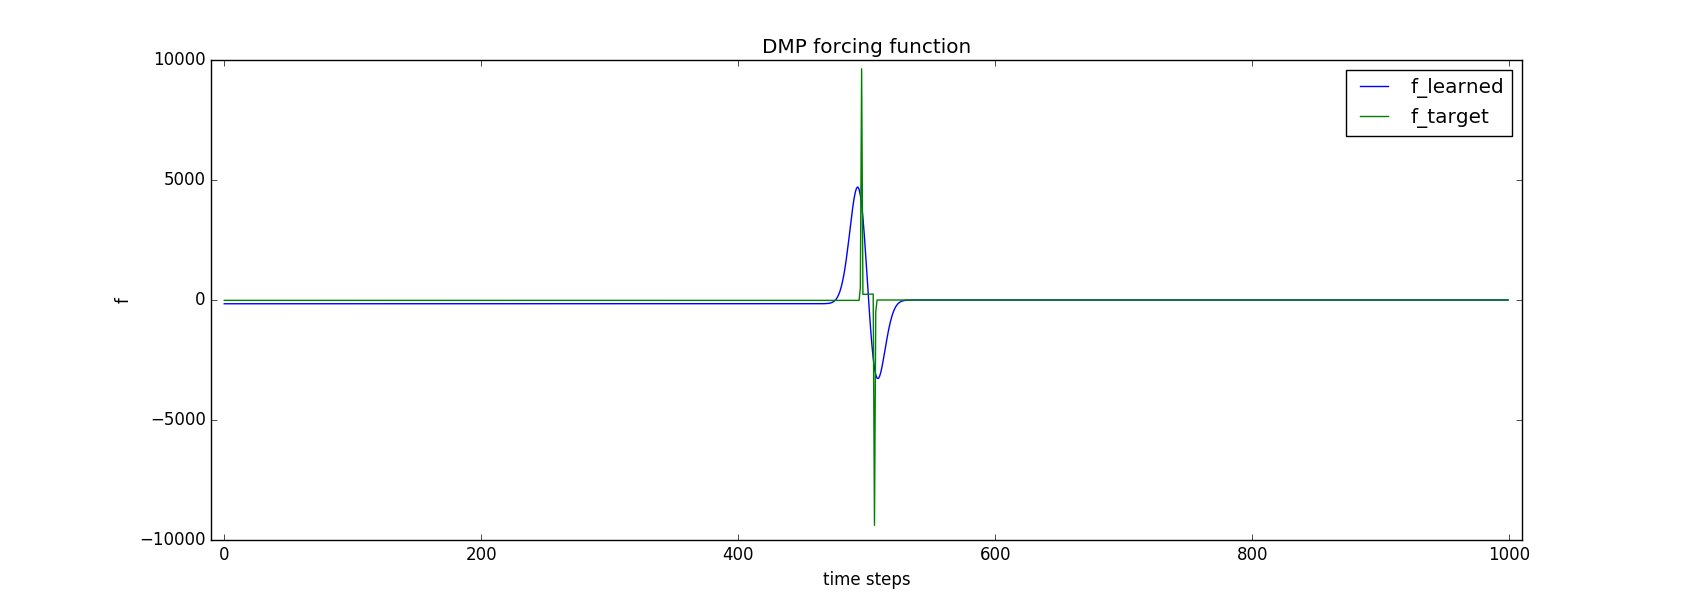
\includegraphics[scale=0.38]{images/f_y.png}
	\caption{Forcing term for y-axis}
	\label{fig:step_f_y}
\end{figure}

 We can observe spikes in both forcing terms, target forcing term and learned forcing term (a positive spike followed by negative spike). As the $f$ is directly added in the acceleration of DMP, positive spike in forcing term produces massive acceleration command in order to achieve step value ($y$ = 1 in this case). Following negative spike brings acceleration back to 0 to settle the $y$ at value 1.   



\begin{figure}[H]
	\centering
	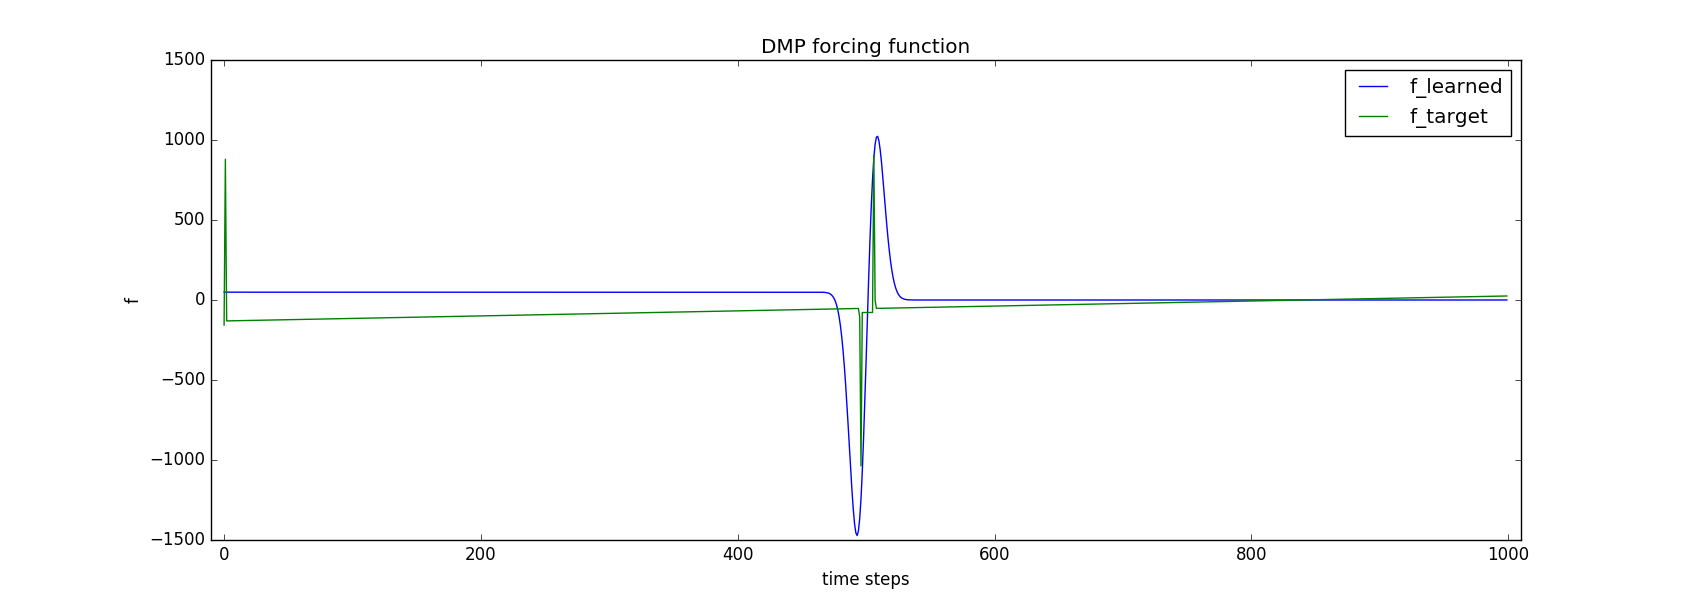
\includegraphics[scale=0.38]{images/f_x.png}
	\caption{Forcing term for x-axis}
	\label{fig:step_f_x}
\end{figure}
At the same time, forcing term associated with DMP in x-axis (shown in fig. \ref{fig:step_f_x}), slows x-velocity down for a while to let $y$ settle at $y = 1$, and then again produces $f$ to attain some velocity to continue till $x = 1$. 

It should be noted that the learned $f$ is relatively smoother than the target forcing function, which introduces error at the corners of the step function trajectory. The smoothness in the learned forcing function depends on number of basis function used.   

Hence in conclusion, DMP learns the shape of trajectories by modifying relative accelerations of individual motion primitives in each degrees of freedom in synchronous fashion. The forcing term associated with each degree of freedom is synchronized with the help of \textit{canonical system}. 

In this project, DMPs are used to learn end-effector motion in Cartesian space. Motion in each degree of freedom is used as separate DMP and then superimposed to create 6D motion. Following figure shows the composition of the motion. Canonical system governs the synchronization between all the degrees of freedoms.

\begin{figure}[H]
	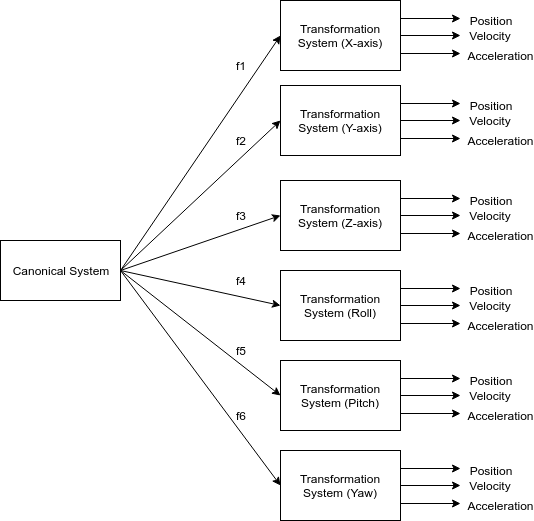
\includegraphics[width=\textwidth]{images/DMP_6DOF.png}
	\caption{6D DMP framework}
	\label{fig:DMP_6DOF}
\end{figure}



\newpage
\subsection{Analysis of the effects of the parameters used in DMP}\label{analysis}
Apart from learning the weights, their are certain parameters in DMP framework which affect the learning and motion generation by DMP. Hence, for better understanding and effective use of DMP, analysis of the effects of these parameters is necessary. 

For analyzing the effects of the various parameters used in DMP, a artificially generated step function trajectory, shown in figure \ref{fig:step_function}, was learned and the parameters were changed in order to evaluate their effects on the DMP. The evaluation criterion was the closeness between the desired path and the path generated by DMP after learning. The error between the path was calculated a as normalized point-to-point distance between the discrete positions on two paths. More precisely , the error was calculated as follows:

\begin{equation}\label{t_error}
	error = \frac{1}{N}\sum_{i = 1}^{N}min\{\norm{P_{i} - Pd_{1}}, \norm{P_{i} - Pd_{2}}, \norm{P_{i} - Pd_{3}}, .... , \norm{P_{i} - Pd_{M}}\}
\end{equation}

Where,\\
$P$ is the path generated by the DMP, \\
$Pd$ is the original demonstrated path, \\
$N$ is the number of poses in $P$, \\
$M$ is the number of poses in $Pd$.


This error function evaluates the closeness of two paths, and hence does not consider the deviation of the trajectory at each time step. It also does not consider the deviation in velocity and acceleration. 

Intuitive analysis of other undesired behaviors such as jumps was also done by observing the paths plotted in 2D graphs.   

The generated artificial trajectory contains 100 2D poses sampled at equal time intervals of 0.01$s$. Values of X and Y coordinate values lie between 0 and 1. Such trajectory cannot be used on a real robot due high values of velocities and accelerations associated with it. But this trajectory is very useful for analysis of DMP system. 

\begin{figure}[H]
	\centering
	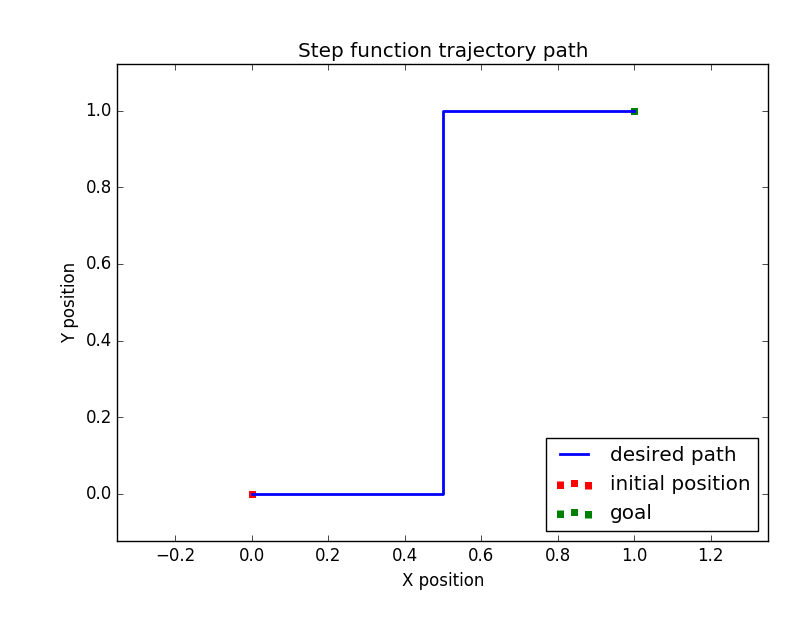
\includegraphics[scale=0.5]{images/step_function.png}
	\caption{Step function trajectory path}
	\label{fig:step_function}
\end{figure}

\subsubsection{Effect of the number of basis functions on the trajectory approximation}

The number of basis functions used in a DMP affects the approximation of the non-linear forcing function which modifies the shape of motion: a higher number of basis functions results in a better approximation of the forcing function. A better approximation of the forcing function means that the shape of the trajectory generated by the DMP will be more similar to the original trajectory which was used for learning. 

Figure \ref{fig:n_bfs_} illustrates the effect of different numbers of basis functions on 
learning the step function trajectory. It can be observed that increasing the number of basis function results in a better approximation of the shape of the original trajectory.  

The error in mimicking the trajectory is summarized in table \ref{_n_bfs_e}. From this data, it can be concluded that the trajectories containing high frequency components can be better approximated with a high number of basis functions.

Fixed parameters : \\
$\tau$ = 1 \\
$dt$ = 0.001

\begin{figure}[H]
	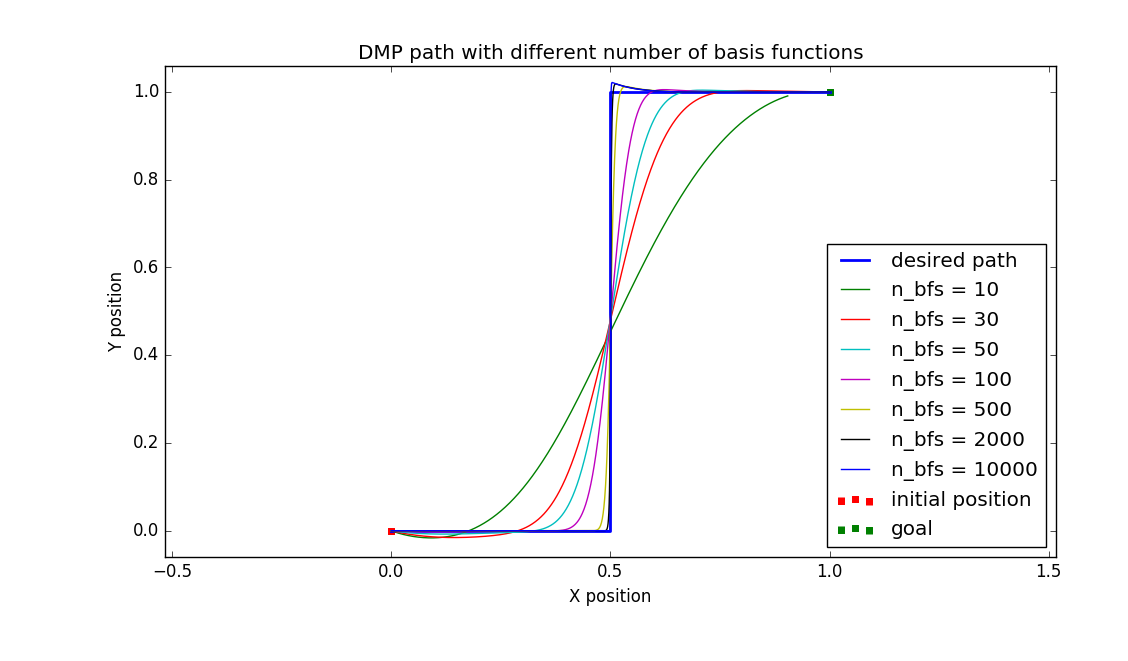
\includegraphics[width=\textwidth]{images/n_bfs_.png}
	\caption{Effect of the number of basis functions ($n\_bfs$) on the trajectory approximation}
	\label{fig:n_bfs_}
\end{figure}



\begin{center}
	\begin{table}[H]
		\begin{tabular}{| c | c | c | c | c | c | c | c |}	
			\hline
			Number of basis functions & 10 & 30 & 50 & 100 & 500 & 2000 & 10000\\       
			\hline
			Error & 0.093 & 0.038 & 0.021 & 0.009 & 0.002 & 0.001 & 0.001\\
			\hline
		\end{tabular}
		\caption{Error in mimicking the trajectory}
	\end{table}\label{_n_bfs_e}
\end{center}



The number of basis functions used while learning the DMP also affects the learning of noise. While demonstrating the trajectory, it is possible that high frequency noise is recorded especially because of vibrations and shaking of the hands of the teacher. If the number of basis function used is very high, the high frequency noise is also learned which may not be desired; low number of basis functions result into a smoother trajectory filtering out the noise. 

The use of high number of basis functions also increases the number of computations at run-time as well as at the time of learning the DMP. As the learning algorithm used is linear and DMPs are learned off-line, the increase in learning time does not matter much, however, if it is required to update the motion commands at high frequency while executing the DMP, using a high number of basis functions is undesirable.     

\subsubsection{Effect of the time step size on the trajectory approximation}   
The motion commands and the trajectory generated by the DMP framework are in discrete time. Euler's integration method is used to solve the differential equations to obtain the kinematic state at each time step; hence, the choice of the step size affects the error in the generated trajectory. If the step size used is not small enough, DMPs can generate trajectories that are potentially undesirable and dangerous to be executed by a robot; in other words, large step sizes result in oscillations in the trajectories. Figure \ref{fig:dt_} illustrates the effect of various time step sizes on the trajectories generated by the DMP framework. 

If the step size is not small enough, the acceleration at a specific point on the trajectory is not updated for long enough time, so that the generated trajectory overshoots and deviates from the desired trajectory. On next time step, a counter acceleration is applied in order to bring the trajectory close to desired trajectory which again overshoot in an opposite direction from the previous time step. This intuitive explanation signifies the need of a small enough time step for a stable behavior of DMPs.   

If the DMP is used for generating instantaneous motion command and feedback from the robot and the environment is coupled with DMP (e.g. position feedback from a robot or obstacles from environment), then it is desirable to keep the time step in the order of $10^{-3}$ to avoid large overshoots. 


Fixed parameters : \\
$n\_bfs$ = 2000 \\
$\tau$ = 1 



\begin{figure}
	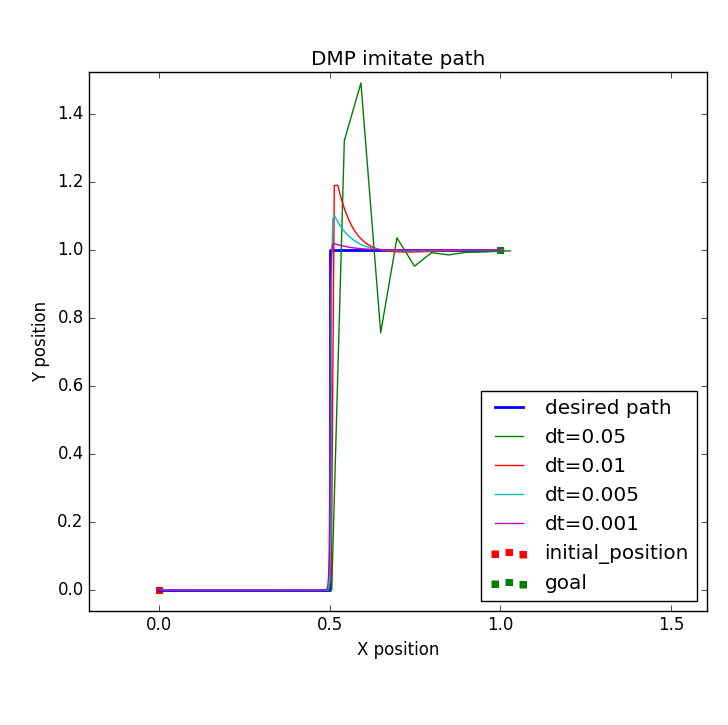
\includegraphics[scale=0.7]{images/dt_.png}
	\caption{Effect of the time step size ($dt$) on the trajectory approximation}
	\label{fig:dt_}
\end{figure}



\begin{center}
	\begin{table}[H]
		\centering
		\begin{tabular}{| c | c | c | c | c | c | c | c |}	
			\hline
			Time step size & 0.05 & 0.01 & 0.005 & 0.001 \\       
			\hline
			Error & 0.062 & 0.017 & 0.011 & 0.007 \\
			\hline
		\end{tabular}
		\caption{Error in mimicking the trajectory}
	\end{table}\label{_dt_e}
\end{center}


\subsubsection{Effect of the time scaling factor $\tau$ on the trajectory approximation}   

The time scaling factor ($\tau$) is used for modifying the speed of the execution of a DMP; in other words, it is a term which scales the acceleration term produced by the transformation system, which in turn results in scaling of the kinematic state at the next time step. If the value of $\tau$ is set to $1$, then the execution speed of DMP is same as that of the demonstration. 

If a large value of $\tau$ is used, undesirable oscillations can be observed in the robot trajectories. The reason behind these oscillations is same as that of the large time step; high values of $\tau$ cause large acceleration at certain time step causing the trajectory to overshoot from the desired path. On next time steps, acceleration in opposite direction is generated by the dynamics of the \textit{transformation system}, which is again scaled by $\tau$ and hence trajectory overshoots in the other direction. The effect of large a $\tau$ can be nullified to a certain extent by choosing a sufficiently small step size. 


Figure \ref{fig:tau_} a illustrates the effect of different values of $\tau$ on DMP. It should be noted that a value of $\tau$ less than 1, does not affect the stability of DMP. Figure \ref{fig:tau_} b shows an unstable behavior of the DMP due to a large value of $\tau$.

Fixed parameters : \\
$dt$ = 0.001 \\
$\tau$ = 1 


\begin{center}
	\begin{table}[H]
		\centering
		\begin{tabular}{| c | c | c | c | c | c | c | c |}	
			\hline
			Time scaling factor ($tau$) & 0.1 & 1 & 10 & 12 & 15 \\       
			\hline
			Error & 0.007 & 0.007 & 0.010 & 0.036 & 0.292   \\
			\hline
		\end{tabular}
		\caption{Error in mimicking the trajectory}
	\end{table}\label{_tau_e}
\end{center}

\begin{figure}[H]
	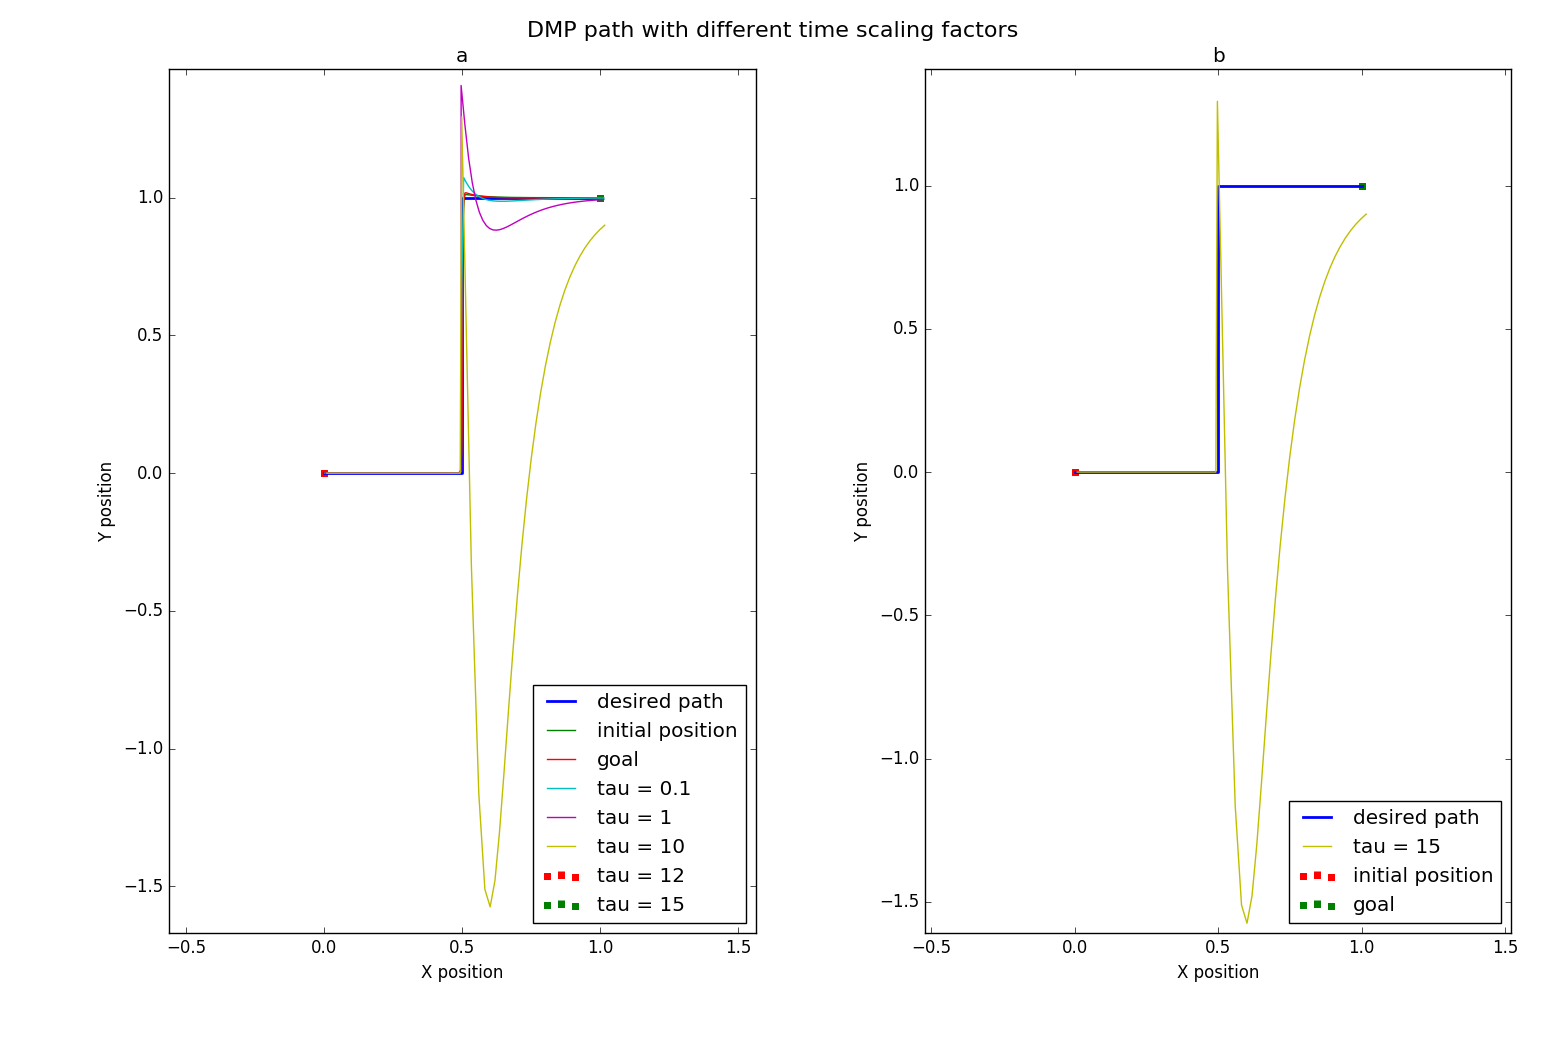
\includegraphics[width=\textwidth]{images/tau_.png}
	\caption{Effect of the time scaling factor $\tau$ on the trajectory approximation}
	\label{fig:tau_}
\end{figure}






\subsection{Demonstration of Trajectories}

In this project, \textit{external observation} method was used to demonstrate the trajectories. In this method, the teacher moves arUco marker board in along the path to be demonstrated. A computer vision system ensures the recording of poses of the arUco marker board in robot \textit{base\_link} frame, at constant rate. 

A \textit{RGB} camera captures the images of demonstration at equal time interval. Each image is processed for estimating 6D pose of the arUco marker board in camera optical frame. 

To estimate the pose of the arUco marker board, \textit{detectMarkers()} and \textit{estimatePoseBoard()} methods in class \textit{aruco} provided by \textit{opencv} library are used. Implementation of these functions are out of the scope of this project. 

These functions internally use \textit{solvePnP()} method which estimates the pose of the local frame of reference in camera optical frame using correspondence between the actual points in the local co-ordinate frame of reference and their projection on the image plane.  

\textit{solvePnP()} function finds such a pose that minimizes re-projection error, that is the sum of squared distances between the observed projections in image and the projected points. For minimization of the error function uses Levenberg-Marquardt optimization method. 

\begin{figure}[H]
	\centering
	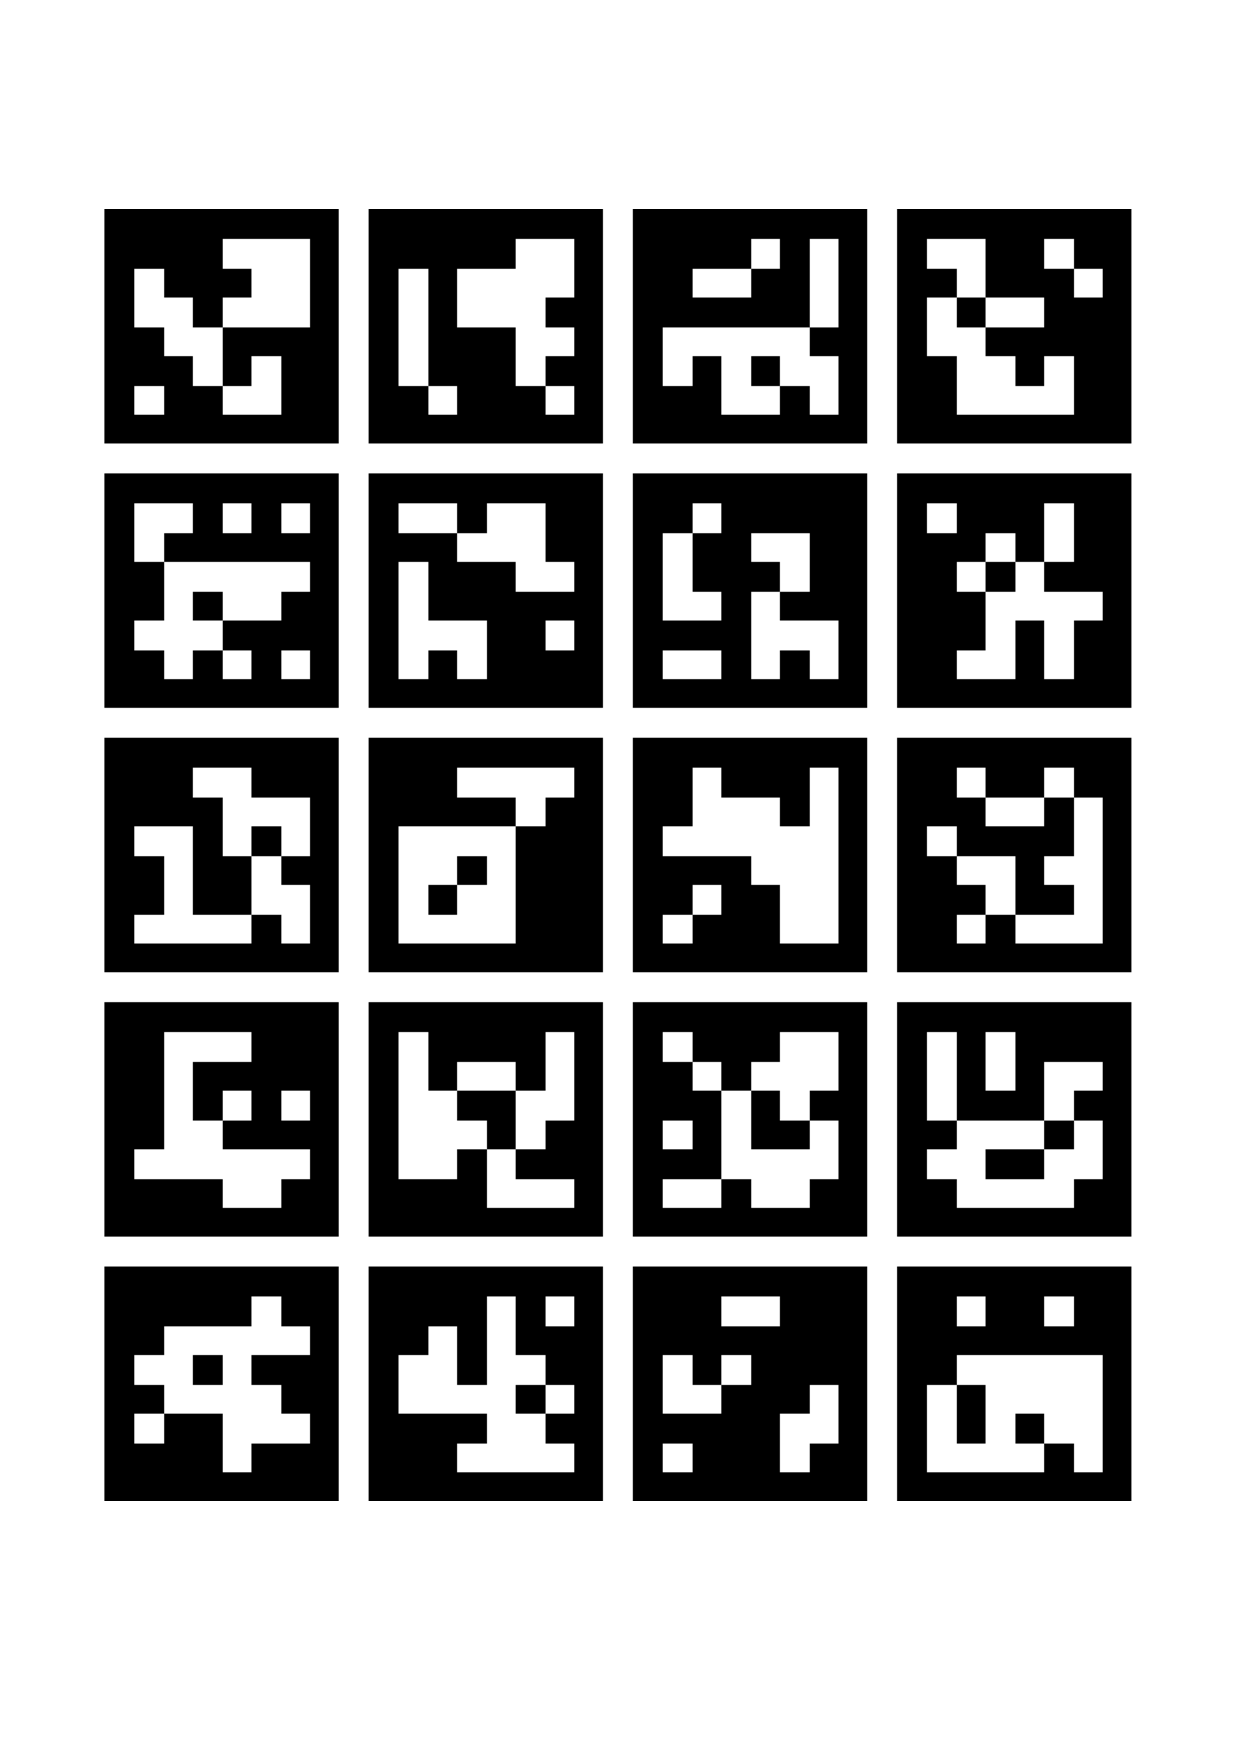
\includegraphics[scale=0.3]{images/aruco_marker_board.pdf}
	\caption{arUco marker board used for demonstrations}
	\label{fig:aruco_marker_board}
\end{figure}

A arUco marker board was used instead of using single arUco marker becuase:\\
\begin{enumerate}
	\item multiple arUco markers on a single board provide more data for pose estimation which results in increased accuracy. 
	\item even if the board is occluded or partially out of field of the view of the camera, it possible to estimate the pose.
	\item due to above reason, it is possible to record poses at almost every discrete time instance, making trajectory continuous in time.
	  
\end{enumerate}
	
This method also has some drawbacks:

\begin{enumerate}
	\item demonstrating rotational motion of end effector is very difficult because it non-intuitive for teacher to rotate the board as if it a end-effector.
	\item while demonstrating the motion, high frequency noise is introduced in the trajectory due shaking of the hands off the teacher.
\end{enumerate}

\subsection{Inverse Kinematics Solver and Trajectory Controller}\label{IK}

In order to execute the task-space trajectory generated by the DMP framework, Cartesian velocities need to be mapped to joint velocities with the help of inverse kinematic solver. The robot arms used in the experiments (a KUKA YouBot arm and Toyota HSR arm) has five degrees of freedom. Five degrees of freedom are not sufficient to carry out a 6 degrees of freedom Cartesian motion at all the time instances. Due to this design deficiency, manipulator is always in the singular configuration. It is well-known that when a manipulator is at-or is in the neighborhood of a singular configuration, severe restrictions may occur on its motion. To overcome this situation, the \textit{weighted damped least square pseudo inverse method} for computing joint velocities was chosen. This method allows us to loose the constraints on the individual degrees of freedom in task-space, which allowed us to ignore the velocity constraints on the 3 rotational degrees of freedom. This is called a user-defined accuracy method to control the manipulator. \cite{chiaverini1994review}


The relation between the joint space and task space velocities can be given by, 

\begin{equation}\label{theta_dot}
	v = J(\theta) \dot{\theta} 
\end{equation}

\begin{equation}\label{theta_dot_inv}
	\dot{\theta} = J(\theta)^{-1}  v
\end{equation} 
Where, \\
$J(\theta)$ is jacobian matrix of manipulator configuration, \\
$v$ is the task space velocity vector, \\
$\dot{\theta}$ is the joint space velocity vector. \\

When a manipulator is near a singularity, Jacobian matrix of the manipulator becomes ill-conditioned. Due to this, "large joint velocities may occur or degenerate directions may exist where end-effector velocity is not feasible"\cite{chiaverini1994review}. To overcome this situation, the damped least square method can be used, where a degraded solution is generated near the singularities proposed in \cite{wampler1986manipulator} and \cite{nakamura1986inverse}. A damping factor is introduced in eq. \ref{theta_dot}; by adjusting the damping factor, resulting Jacobian matrix can be made well-conditioned. 

The equation \ref{theta_dot} is modified by introducing a new term $\lambda$ called damping factor,

\begin{equation}\label{damped_least}
	J^{T}(\theta)v = (J^{T}(\theta)J(\theta) + \lambda ^{2}I)\dot{\theta}
\end{equation}

Where, \\
$\lambda > 0 $ is a damping factor, and \\
$I $ is identity matrix. 

The solution to above problem is, 
\begin{equation}\label{damped_least_sol}
	\dot{\theta} = (J^{T}(\theta)J(\theta) + \lambda^{2}I)^{-1}J^{T}(\theta)v
\end{equation} 

It should be noted that if the value of $\lambda$ in eq. \ref{damped_least_sol} is set to 0, eq. \ref{damped_least_sol} reduces to eq. \ref{theta_dot_inv}.

Eq. \ref{damped_least} satisfies the condition,

\begin{equation}
	\underset{\dot{\theta}}{min}(\norm{v - J(\theta)\dot{\theta}}^{2} + \lambda^{2}\norm{\dot{\theta}})
\end{equation}

which evidences the possibility of trading off accuracy against feasibility of the joint velocity required to generate the given end-effector velocity. Therefore, it is essential to select suitable values for the damping factor: Small values of $\lambda$ give accurate solutions but low robustness to the occurrence of singular and near-singular configurations. Large values of $\lambda$ result in low tracking accuracy even when a feasible and accurate solution would be possible\cite{chiaverini1994review}.

The effect of the value of $\lambda$ on joint velocities can be analyzed further by the singular value decomposition. Using singular value decomposition, equation \ref{damped_least_sol} can be re-written as,

\begin{equation}
\dot{\theta} = \sum_{i=1}^{6}\frac{\sigma_{i}}{\sigma_{i}^{2} + \lambda^{2} }\textbf{v}_{i}u_{i}^{T}v
\end{equation} 

In above equation, it can be observed that, if $\sigma \gg \lambda$, then $\lambda$ has practically no effect on the joint velocities. But if $\sigma$ is close to zero, then the joint velocities are greatly affected by the value of $\lambda$. The damping factor determines the degree of approximation introduced with respect to the pure least-squares solution.

Since the arm has only five degrees of freedom, it is always in singular configuration and hence it is not possible to execute the 6 degrees of motion at all the time instances. This situation can be overcome by ignoring motion in specific rotational degrees of freedom with the help of the method called \textit{weighted damped least square pseudo inverse}. In this method, Cartesian velocities are multiplied by a weighting matrix. 

\begin{equation}
	\tilde{v} = \text{W}v
\end{equation}
where $\text{W}$ is the (6 x 6) task-space weighting matrix\cite{wampler1986manipulator}.

Substituting $\tilde{v}$ in eq. \ref{theta_dot}, we get,

\begin{equation}
\tilde{v} = \tilde{J(\theta)}\dot{\theta} 
\end{equation}

Where, $\tilde{J(\theta)} = \text{W}J(\theta)$ \\

In other words, by choosing appropriate W, ill-conditioned matrix $J$ an be made well conditioned. Here we need to sacrifice the accuracy on particular degree of freedom which depends of choice of W. Further use of damped least square method described above will generate more feasible solutions for joint velocity. 

\subsection{Whole Body Motion}\label{whole_body_motion}

For the robotic manipulators with limited capabilities in terms of reachable workspace, it is not possible to execute the trajectory generated by a DMP which is outside the dexterous workspace. Hence it becomes necessary to use navigation functionality of the mobile platform on which manipulator is fixed in co-ordination with the manipulator's end-effector motion to track the Cartesian trajectories by end-effector of the manipulator. Such integration of motion of base platform and motion of manipulator end-effector can be called as \textit{whole body motion}.  

To implement the whole body motion control, first a policy should be devised which will govern the distribution of motion between manipulator and mobile base platform. This policy should be able to co-ordinate and synchronize the motion executed by mobile base and manipulator. The necessary requirement for such policy design is to identify the capability of manipulator to execute instantaneous motion at each point in time. This capability can be judged by observing the singular values of manipulator's Jacobian matrix.

When a manipulator end-effector is operating near the boundary of reachable workspace, a velocity command which drives end-effector towards the boundary makes the Jacobian matrix of the manipulator more ill-conditioned and smallest singular value obtained by singular value decomposition of Jacobian matrix, tends to zero\cite{wampler1986manipulator}. In other words, a manipulator's capability of executing motion commands in the direction towards the boundary of work-space decreases with decreasing value of smallest singular value. It should be noted that, velocity commands driving manipulator end-effector away from the boundary inside the reachable workspace, can be executed normally.    

In this project, a linear motion distribution policy was developed which calculates the velocity commands for the base and manipulator end-effector by observing the smallest singular value of Jacobian matrix of the manipulator. The singular values can be obtained as follow:

The relation between the joint-space velocities and Cartesian velocities is given by equation \ref{theta_dot}, which is 

\begin{equation}
	v = J(\theta) \dot{\theta} 
\end{equation}
Where, \\
$v$ is the velocity vector in global co-ordinate frame. 

Singular values of Jacobian can be obtained by singular value decomposition,

\begin{equation}
	J = \sum_{i=1}^{6}\sigma_{i}u_{i}\textbf{v}_{i}^{T}
\end{equation}   

Where, $\sigma_{i}$ are the singular values. 

The policy for distribution of linear velocities amongst the mobile base platform and manipulator end-effector is given by,

\begin{equation}
	m_{cap} = \frac{(\sigma_{min} - \sigma_{l})}{(\sigma_{h} - \sigma_{l})}
\end{equation}

\begin{equation}
	v_{ee} = m_{cap}.v
\end{equation} 

\begin{equation}
	v_{b} = (1 - m_{cap}).v
\end{equation} 
Where, \\
$m_{cap}$ is capability co-efficient of manipulator, \\
$\sigma_{min}$ is the smallest singular value, \\
$\sigma_{l}$ is the lower limit on $\sigma_{min}$, \\
$\sigma_{h}$ is the upper limit on $\sigma_{min}$, \\
$v$ is the desired linear velocity of manipulator end-effector in global frame of reference, \\ 
$v_{ee}$ is the velocity command for end-effector in global frame of reference, \\
$v_{b}$ is the velocity command for mobile base in global frame of reference.


It should be noted that above policy comes into effect only when $\sigma_{min} \le \sigma_{h}$. Also, only linear motion is distributed between mobile base and manipulator end-effector, rotational motion is executed by the manipulator only.


It is also possible that in the environment in which the robot is operating, motion of the mobile base is not possible in particular direction because of the obstacles. Hence it is necessary to incorporate this information while distributing the motion commands. Above policy can be modified as follow to accommodate the constraints on the base movement.


\begin{equation}
m_{cap} = \frac{(\sigma_{min} - \sigma_{l})}{(\sigma_{h} - \sigma_{l})}
\end{equation}


\begin{equation}
b_{cap} = \frac{(d - d_{l})}{(d_{h} - d_{l})}
\end{equation}


\begin{equation}
v_{ee} = \frac{m_{cap}}{m_{cap} + b_{cap}}.v
\end{equation} 

\begin{equation}
v_{b} = \frac{b_{cap}}{m_{cap} + b_{cap}}.v
\end{equation} 

Where, \\
$m_{cap}$ is capability co-efficient of manipulator, \\
$\sigma_{min}$ is the smallest sigma value, \\
$\sigma_{l}$ is the lower limit on $\sigma_{min}$, \\
$\sigma_{h}$ is the upper limit on $\sigma_{min}$, \\
$b_{cap}$ is capability co-efficient of mobile base, \\
$d$ is the distance of the obstacle from base, \\
$d_{l}$ is the lower limit on $d$, \\
$d_{h}$ is the upper limit on $d$, \\
$v$ is the desired velocity of end-effector in global frame of reference, \\ 
$v_{ee}$ is the velocity command for end-effector of the manipulator in global frame of reference, \\
$v_{b}$ is the velocity command for mobile base in global frame of reference.

Here, if the sum ($m_{cap} + b_{cap}$) drops below certain threshold value, it can be concluded that the further motion is not possible, as both the motion capabilities are reduced significantly. 